\chapter{Bayesian Neural Networks}
% Authors: Jong Yeob Kim (editor), Zilin Bian, Di Sha, 4/23/19.

\section{ Motivation of estimating a predictive distribution }

Most of modern neural network models produce point estimation, even though at last phase of image classification models we get confidence scores of different categories like cat and dogs. With complexity/uncertainties happening all the time around the world, it is not always reasonable to get a single output result. Sometimes we cannot tell whether the new model is making sensible predictions or just guessing at random. In this situation, we may wish to get a predictive distribution of results instead of a point estimation.\\

\section{Motivation of caring about uncertainty}

Given several pictures of cats and dogs, then being asked to classify a new cat photo, we should return a prediction with rather high confidence. But if we are given a photo of an ostrich and force our hand to decide if it is a cat or dog, we should return a prediction with very low confidence. It is quite important to say whether we are confident about our estimation or not. Another example is predicting physics simulator. In physics, you may have simulators for predicting the trajectory of some particles or accelerators. But, then this simulation takes forever. In this case, you can use neural networks to speed up computations and getting approximate values. The network is trained over many iterations using data provided by simulators. However, if inputs are far from trained data, a prediction is made with higher uncertainty. Furthermore, this sort of information lies at the foundations of artificial intelligence as well. For example, a Roomba vacuum needs to learn about its environment (e.g. living room) based on its actions (rolling around in different directions). It can decide to go forward and might bump into a wall. One should enable reward mechanism to encourage it when it learns to avoid the wall or penalize it when it crahses into a sofa. This setting is known as reinforcement learning. The Roomba is requried to explore its environment looking for these rewards, and that's where uncertainty comes into play. The Roomba will try to minimise its uncertainty about different actions - and trade-off between this exploration, and exploitation of what it already knows. You can trace to Karpathy's (https://cs.stanford.edu/people/karpathy/convnetjs/demo/rldemo.html) interactive demo to learn into this Roomba play. 

\section{Get predictive distribution using dropout}

Take any network trained with dropout and some input $x^*$. We are looking for the expected model output given our input - the predictive mean $\mathbb{E}(y^*)$ and how much the model is confident in its prediction - the predictive variance $Var(y^*)$. The neural network model with enabled dropout in both train and test phases will be equivalent to Gaussian process approximation. In the following section we will walk through the process of enabling dropout and getting the estimation of predictive distribution.\\
First, define a prior length-scale $l$. This captures our belief over the function frequency. A short length-scale $l$ corresponds to high frequency data, and a long length-scale corresponds to low frequency data.Take the length-scale squared, and divide it by the weight decay. We then scale the result by half the dropout probability over the number of data points. Mathematically this result in a Gaussian process precision $\tau = \frac{l^2 p}{2N \lambda}$ we mentioned above. Note that $p$ here is the probability of the units not being dropped - in most implementations $p_{code}$ is defined as the probability of the units to be dropped, thus $p := 1- p_{code}$ should be used when calculating $\tau$. Next, simulate a network output with input $x^*$, treating dropout as if we were using it during training phase. This means enabling dropout also in test phase. Repeat this $T$ times with different units dropped every time, and collect the results ${\hat{y_t}^* (x^*)}$. These are empirical samples from our approximate predictive posterior. We can get an empirical estimator for the predictive mean of our approximate posterior as well as the predictive variance (our uncertainty) from these samples. Mathematically, averaging forward passes through the network is equivalent to Monte Carlo integration over a Gaussian process posterior approximation. The derivation is provided in \cite{gal2016dropout}. The process of applying dropout into the neural network at both training and test phases is thus called Monte-Carlo dropout (MC dropout). We simply follow these two equations:
\begin{equation}
    \mathbb{E} (y^*) \approx \frac{1}{T} \sum^{T}_{t=1} \hat{y_t}^*(x^*)
\end{equation}
\begin{equation}
    Var(y^*) \approx \tau^{-1} I_D + \frac{1}{T}\sum^{T}_{t=1} \hat{y_t}^*(x^*)^T \hat{y_t}^* (x^*) - \mathbb{E} (y^*)^T \mathbb{E} (y^*)
\end{equation}
\\
Eq. 17.1 was introduced as model averaging and it was explained that scaling the weights at test time without dropout gives a reasonable approximation to this equation. Eq. 17.2 is simply the sample variance of $T$ forward passes through the network plus the inverse model precision. Note that the vectors above are row vectors and that the products are outer-products.
\\
Implementation in python code to get the predictive mean and uncertainty is easy:
\begin{figure}[H]
    \centering
    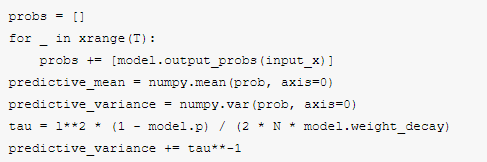
\includegraphics[width=\textwidth]{labs/12/images/python code of getting mean and var.PNG}
    \caption{Python code to obtain predictive mean and uncertainty from dropout}
    \label{fig:visual_caption}
\end{figure}

\section{Understanding MC dropout Models}
\subsection{Regression}
To see what the uncertainty looks like where points are far away from training data, we can visualize it using a simple one dimensional regression model with a subset of the atmospheric CO$_2$ concentrations dataset. This dataset was derived from situ air samples collected at Mauna Loa Observatory, Hawaii, since 1958. The dataset consists of about 200 data points and has been centered and normalized. Fig. \ref{fig:co2_concentration} shows the raw data, and \ref{fig:regression_without_uncertainty} shows the processed training data (in red, left of the dashed blue line) and a missing section to the right of the dashed blue line. A neural network with 5 hidden layers, 1024 units in each layer, and ReLU non-linearities, and dropout with probability 0.1 after each weight layer, was fitted to the data.

\begin{figure}[H]
    \centering
    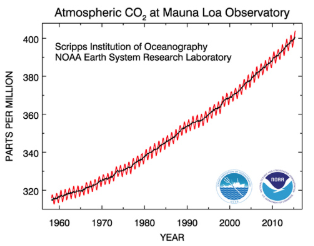
\includegraphics[width=10cm]{labs/12/images/CO2 concentration.png}
    \caption{CO$_2$ dataset before pre-processing}
    \label{fig:co2_concentration}
\end{figure}

\begin{figure}[H]
    \centering
    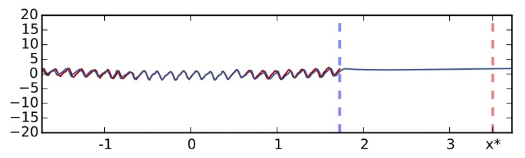
\includegraphics[width=10cm]{labs/12/images/Regression without uncertainty.png}
    \caption{Standard dropout network without using uncertainty information}
    \label{fig:regression_without_uncertainty}
\end{figure}

The point marked with a dashed red line is a point far away from the training data. As can be seen, standard dropout confidently predicts a clearly insensible value for the point, as the function is obviously periodic. Therefore, it is really hard to tell whether the model can be trusted or not. However, if we add the uncertainty information introduced above to the exactly same network (we don't need to re-train the model, just perform predictions in a different way), we can get the revealing information shown in Fig. \ref{fig:regression_with_uncertainty}.

\begin{figure}[H]
    \centering
    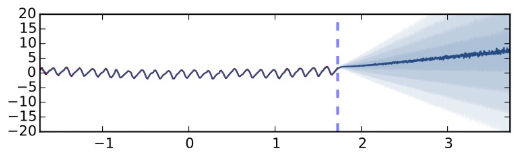
\includegraphics[width=10cm]{labs/12/images/Regression with uncertainty.png}
    \caption{Same dropout network performing predictions using uncertainty information}
    \label{fig:regression_with_uncertainty}
\end{figure}

As can be seen, the model does capture a large amount of uncertainty information about the far away test point. This uncertainty information is very similar with that of a Gaussian process model with a squared exponential covariance function (as shown in Fig. \ref{fig:regression_GP}). Though the estimate is different, the uncertainty still increases as the test point goes farther from the training data. It's not surprising that the uncertainty looks different, since the ReLU non-linearity corresponds to a different Gaussian process covariance function. If we change the non-linearity to a TanH non-linearity, the result looks as shown in Fig. \ref{fig:regression_tanh}.

\begin{figure}[H]
    \centering
    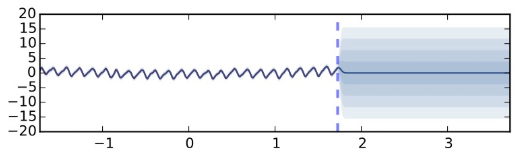
\includegraphics[width=10cm]{labs/12/images/Regression using Gaussian Process.png}
    \caption{Gaussian process with SE covariance function on the same dataset}
    \label{fig:regression_GP}
\end{figure}

\begin{figure}[H]
    \centering
    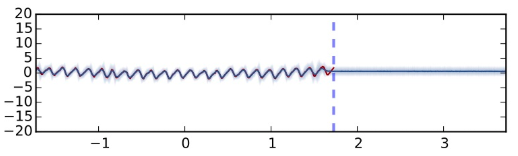
\includegraphics[width=10cm]{labs/12/images/Regression using TanH.png}
    \caption{Dropout network using uncertainty information and TanH non-linearity}
    \label{fig:regression_tanh}
\end{figure}

This time it seems that the uncertainty doesn't increase as farther from the training data. This might be because TanH saturates whereas ReLU does not. This non-linearity will not be appropriate for tasks where we are expecting the uncertainty to increase as the test point goes farther away from the training data.

\subsection{Classification}
This section takes an example of image classification using MNIST digits dataset and the popular LeNet convolutional neural network. In this model the prediction is fed into a softmax which gives probabilities for different classes (the 10 digits). However, these probabilities are not enough to see if the model is certain in its prediction or not. This is because the standard model would pass the predictive mean through the softmax rather than the entire distribution.

If we take an idealized binary classification example (as shown in Fig. \ref{fig:classification_binary}). Passing a point estimate of the mean of a function (a TanH function for simplicity, solid line on the left) through a softmax (solid line on the right) results in highly confident extrapolations with $x^*$ (a point far from the training data) classified as Class 1 with probability 1. However, passing the distribution (shaded area on the left) through a softmax (shaded area on the right) reflects classification uncertainty better at points far from the training data. Taking the mean of this distribution passed through the softmax we get Class 1 with probability 0.5 -- the model's true prediction.

\begin{figure}[H]
    \centering
    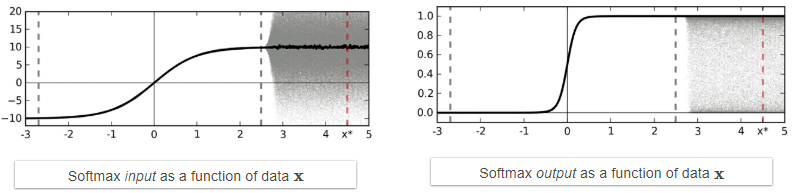
\includegraphics[width=\textwidth]{labs/12/images/Classification_binary.png}
    \caption{A sketch of softmax input and output for an idealized binary classification problem}
    \label{fig:classification_binary}
\end{figure}

Then we can try passing the entire distribution through the softmax instead of the mean alone. The samples are simulated through the network and the softmax output is averaged. The convolutional neural network is trained over MNIST with dropout applied after the last inner-product layer (with probability 0.5). The model predictions are evaluated over the following sequence of images (Fig. \ref{fig:classification_input}), that correspond to some projection in the image space.

\begin{figure}[H]
    \centering
    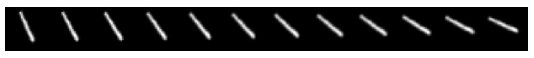
\includegraphics[width=10cm]{labs/12/images/Classification_input.png}
    \caption{Image inputs (a rotated digit) to the dropout LeNet network}
    \label{fig:classification_input}
\end{figure}

These images correspond to the $X$ axis in the idealized depiction above. A histogram of 100 samples obtained by simulating forward passes through the dropout LeNet network is shown in Fig. \ref{fig:classification_multi}. As can be seen, Class 7 has low uncertainty for the right-most images. This is because the uncertainty ``envelope" of the softmax input for these images is far away from the envelopes of all other classes. In contrast, the uncertainty envelope of Class 5 for the middle images interests the envelopes of some of the other classes (even though its mean is higher) -- resulting in large uncertainty for the softmax output. It is important to note that the model uncertainty in the softmax output can be summarized by taking the mean of the distribution. In the idealized example above, this would result in softmax output 0.5 for point $x^*$ (instead of softmax output 1) and here it will result in a lower softmax output that might result in a different image class. This sort of information can help us in classification tasks: obtaining higher classification accuracies. It also helps us analyze our model and decide whether we have enough data or if the model is specified correctly.

\begin{figure}[H]
    \centering
    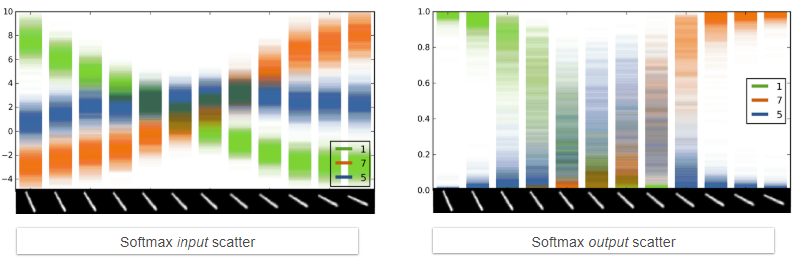
\includegraphics[width=\textwidth]{labs/12/images/Classification_multi.png}
    \caption{A sketch of 100 forward passes of the softmax input and output for dropout LeNet}
    \label{fig:classification_multi}
\end{figure}